\documentclass{book}
\usepackage{graphicx}
\usepackage{xeCJK}
\usepackage{wrapfig}
\setCJKmainfont{WenQuanYi Micro Hei}
\begin{document}

\begin {figure}[H]
  \centering
  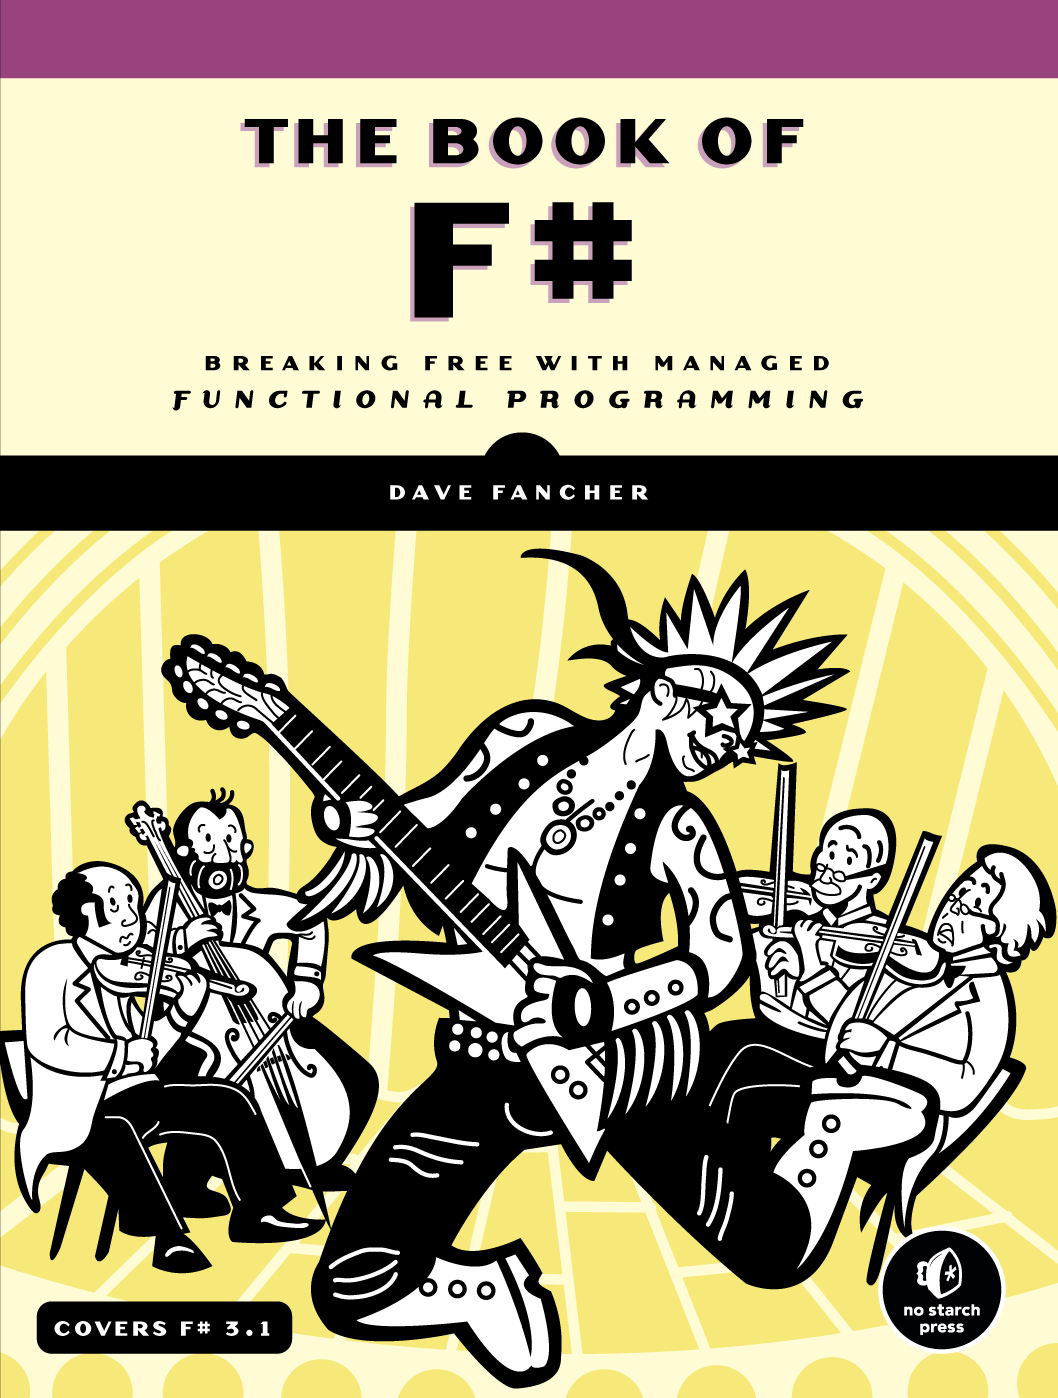
\includegraphics[width=\paperwidth,height=\paperheight]{../pic/cover.png}
  \caption{Endpoint detection}
\end {figure}

The Book of F\#
\title{The Book\\of F\\Breaking Free with Managed \\Functional Programming}
\author{by Dave Fancher}
\maketitle


San Francisco



The Book of F\#. Copyright © 2014 by Dave Fancher.
All rights reserved. No part of this work may be reproduced or transmitted in any form or by any means, electronic
or mechanical, including photocopying, recording, or by any information storage or retrieval system, without the
prior written permission of the copyright owner and the publisher.
Printed in USA
First printing
18 17 16 15 14   1 2 3 4 5 6 7 8 9
ISBN-10: 1-59327-552-8
ISBN-13: 978-1-59327-552-5
Publisher: William Pollock
Production Editor: Alison Law
Cover Illustration: Chris Gould
Interior Design: Octopod Studios
Developmental Editors: Seph Kramer and William Pollock
Technical Reviewers: Kevin Miller and Tomas Petricek
Copyeditor: Rachel Monaghan
Compositors: Laurel Chun and Susan Glinert Stevens
Proofreader: James Fraleigh
For information on distribution, translations, or bulk sales, please contact No Starch Press, Inc. directly:
No Starch Press, Inc.
245 8th Street, San Francisco, CA 94103
phone: 415.863.9900; fax: 415.863.9950; info@nostarch.com; www.nostarch.com
Library of Congress Cataloging-in-Publication Data
Fancher, Dave.
The book of F\# : breaking free with managed functional programming / by Dave Fancher.
pages cm
Includes index.
ISBN 978-1-59327-552-5 -- ISBN 1-59327-552-8
1. F\# (Computer program language) I. Title. II. Title: Book of F-sharp.
QA76.73.F163F36 2014
005.1'17--dc23
2014000831
No Starch Press and the No Starch Press logo are registered trademarks of No Starch Press, Inc. Other product and
company names mentioned herein may be the trademarks of their respective owners. Rather than use a trademark
symbol with every occurrence of a trademarked name, we are using the names only in an editorial fashion and to
the benefit of the trademark owner, with no intention of infringement of the trademark.
The information in this book is distributed on an “As Is” basis, without warranty. While every precaution has been
taken in the preparation of this work, neither the author nor No Starch Pa4paperress, Inc. shall have any liability to any
person or entity with respect to any loss or damage caused or alleged to be caused directly or indirectly by the infor-
mation contained in it.

\newpage{}

\begin{wrapfigure}{r}{5cm}
  
\includegraphics[width=5.0cm]{../pic/Author.png}
\end{wrapfigure}
\paragraph{\textbf{About the Author}}
Dave Fancher has been developing software with the .NET Framework for more than a decade. He is a familiar face in the Indiana development community as both a speaker and participant in user groups around the state. In July 2013, Dave was recognized as a Microsoft MVP (Most Valuable Professional) for Visual F\#. When not writing code or writing about code at davefancher.com, he can often be found watching a movie or gaming on his Xbox One.


\begin{wrapfigure}{r}{5cm}
  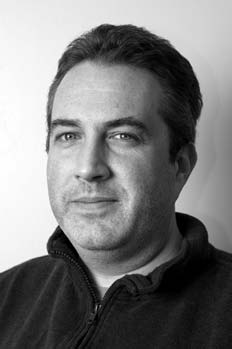
\includegraphics[width=5.0cm]{../pic/KevinMiller.png}
\end{wrapfigure}
\paragraph{\textbf{About the Technical Reviewer}}
Over the last 14 years, Kevin Miller hasa4paper worked on exciting projects with truly great people while unsuccessfully pleading with compilers to break their steadfast rules. He enjoys studying the inherent beauty of logic, and when inspired by the muses, actually codes something deserving a modicum of pride from time to time. His interests lie in security, distributed systems, and data, but he has a short attention ... squirrel!


\end{document}
